%%==================================================
%% chapter03.tex for SJTU Master Thesis
%% Encoding: UTF-8
%%==================================================

\chapter{Trivium算法在物联网中的应用}
\label{chap:use}

在第二章中,本文详细讨论了Trivium算法的结构和一些设计准则。现在本文要考查Trivium算法是否能在物联网中胜任加密算法一职。因此本章将首先讨论Trivium算法在物联网中的优势,然后给出一个假想的应用场景下Trivium算法的完整的应用。

\section{Trivium算法的优势}
\label{sec:advantage}

\subsection{高效性}

考虑到对物联网的一个期望是未来能够实现自动化,那么对于实时性就有很高的要求,这样才能保证各物品之间相互的协调能不出错,因此作为要在物联网中使用的加密算法,首当其冲的要求就是加密算法的高效性了。Trivium算法作为加密算法的高效性的一个保证就是其是流密码,流密码本身就具有实现简单、便于硬件实现、加密解密速度快、低错误传播等特点,因此作为流密码一种的Trivium算法自然也具备这些特点。

当然,流密码内部也有速度的优劣之分。一般而言,要提升流密码算法的效率有两种方法:第一种方法是尽可能减少逻辑门数,使整体结构更为紧凑;第二种方法是改变传统流密码每个cycle只产生一位密钥的做法,转为每个cycle产生多位密钥。显然,这两种做法各有优劣,第一种减少逻辑门数使结构紧凑的做法不适用于要求高速加密的环境,即产生同样位数的密钥需要更少的cycle;而第二种一次cycle产生多位密钥的做法则不适用于要求紧凑结构的环境,比如芯片大小的限制。

Trivium算法并没有固定使用上述的两种方法的某一种,而是一种可变结构,能够成为上述两种两种方法的任意一种。一般提到的Trivium算法属于第一种方法,共使用3488个逻辑门,每个cycle产生一位密钥,但是因为至少要64个cycle才有可能使每个内部状态位被使用,因此可以并行地一个cycle产生64位密钥,此时共使用5504个逻辑门。可见Trivium算法可以适应不同的加密速度或空间的要求。

另外根据eSTREAM的分析,在x86平台加密大块数据时,Trivium算法的效率大约为4 cycles/byte,而在同样平台上,AES的效率大约为19 cycles/byte,可见Trivium算法的高效性。

\subsection{安全性}

既然期望中的物联网是物物相连,那么必然与我们的日常生活的联系比起现在的互联网会更加紧密,自然对于安全的要求更不可忽略。这里又要提到流密码的特点,在1949年Shannon证明了只有一次一密的密码体制是绝对安全的,而“一次一密”正式流密码的密码方案雏形,如果流密码的密码流是真正随机且和消息流长度相同的话,这时的流密码就是一次一密的密码体制。

当然这并不是说Trivium就绝对安全了,事实上,对于Trivium算法已经有不少的攻击研究了。虽然目前对Trivium算法最有效的攻击仍是暴力破解,但也有不少其他方案很接近了。例如,Michael Vielhaber曾针对将初始化状态更新次数降至576轮的变种Trivium算法用仅仅$2^{12.3}$步攻破\parencite{cryptoeprint:2007:413}。于是,其他一些作者基于此猜测使用这种攻击技术可能可以攻破1100轮初始化状态更新次数的Trivium算法甚至攻破原本的Trivium算法\parencite{cryptoeprint:2008:385}。之后,有人得到了需要$2^{68}$步来攻破的针对一种将初始化状态更新次数降至799轮的变种Trivium算法的立体攻击\parencite{cryptoeprint:2015:312}。另一种攻击使用大约$2^{89.5}$步(每步都约为一个简单的穷举算法的量级)恢复了所有寄存器的内部状态,即也能找到密钥\parencite{cryptoeprint:2007:021}。基于同样的原理,被削弱的变种Trivium算法通过一种被称为equation-solving的技术攻破\parencite{raddum2006cryptanalytic}。Trivium算法共288位内部状态,因此照理应需要$2^{144}$步才能攻破,而这些攻击通过改良在流密码攻击中的时间空间权衡,表明如果仅仅对Trivium算法增加密钥长度,而非做其他改变,那么Trivium算法仍不会安全。

但是,虽然上述这些描述看似Trivium算法被攻破指日可待,但其实并不一定如此。首先,虽然比起原本需要$2^{144}$步而言,这些攻击确实大大降低了时间空间消耗,但他们需要的计算量级仍然不可以说是任何人都能做到的,而且也无法保障在攻击期间不会更换密钥,只要更换密钥的周期小于攻击的时间一样能保障安全。另外值得注意的是,所谓的攻击,并非就直接给一个使用Trivium算法的设备,然后就让研究者攻击,而是都会做很多假定,比如有的假定把Trivium算法初始的内部状态更新轮数减少,有的假定可以操纵明文的输入,有的假定可以随时看到内部状态,有的假定甚至可以更改一两位内部状态,这些假定使这些攻击得以成立,但并不是说实际应用中就能实现。比如Trivium算法初始的内部状态更新轮数,这个肯定不是随便一个厂商能自己决定改的。再比如物联网中实际用的时候很多物品如果要通信,那使用的肯定都是固定的一些消息,而不可能是用户都能自己规定,这样自己操纵明文这块也走不通了。比较可行的是看内部状态或者修改内部状态这种,但实际上Trivium算法是硬件实现,速度非常快,是否能真的导出实时内部状态或修改也是一大问题。

因此,既然至今为止对Trivium算法最有效的攻击手段仍是暴力破解,那么至少在当下Trivium算法的理论安全性是可以有保障的,因此使用Trivium算法时要注意的安全问题应该是密钥和初始向量的选取,上述章节中也提到可以构建出小周期的初始内部状态,那么要保障Trivium算法的安全性就应该避免初始内部状态落在这些可以简单构建出的能产生小周期的初始内部状态中,譬如,Trivium算法要求初始内部状态末尾是3个1,这就很有效地防止了会产生周期为3的初始内部状态的出现。因此,现阶段可以做一个类似黑名单的机制,把那些能产生小周期的初始内部状态放在黑名单中,避免使用他们,又或者如果能反其道而行,找到能构建出产生大周期的内部状态的方法,那也可以有效保障Trivium算法的安全性。

\section{贵重物品追踪}

由于时间有限以及没有相应的设备以供尝试实现,本文仅假象应用场景,并加以探讨理论上的设计原理及设计方案,而非实际实现并在真实设备上加以测试。


\subsection{背景}

如前文所述,早期对物联网的定义为在计算机互联网的基础上,利用RFID、无线数据通信等技术,构造一个覆盖世界上各种事物的网络,以实现自动识别物品和互联共享信息。而RFID现在被广泛利用在物流领域,其中便有利用RFID进行贵重物品追踪这一想法诞生。譬如某商场订购了一台电梯,而电梯由各个小零件组成,需要到现场安装,这就涉及如何保证到达现场后各零件都没有遗失,一个做法就是对某个零件都贴上一个标签,然后可以实时追踪这些零件是否在一起,是否到达现场,并且到达现场后进行扫描查看是否有遗漏。又或者是珠宝店需要运输一批珠宝到店里,需要保证运输途中没有遗失,需要实时监控运输到何处。可见贵重物品追踪这一概念是属于物联网领域的,而且也很适合现在仍处于起步阶段的物联网实现。虽然看上去贵重物品追踪好像和我们的日常生活没什么联系,毕竟大部分人并没有运输贵重物品的需求,但其实并非如此,现在人们对淘宝、京东等各大电商肯定不会陌生,网购也成为很多人生活的一部分,而网购自然免不了送货或者说物流这一块,这时使消费者购买的物品能被消费者实时追踪所在何处不就是贵重物品追踪这一概念的推广吗。

当然,贵重物品追踪中也少不了安全需求,其中最重要的一项需求就是如何保证物品的位置信息只被该看的人看到。试想,如果物品的位置信息能够被别人轻易拿到,那么如果运输的是贵重物品,那么反而让犯罪分子能实时追踪到目标;如果运输的是消费者的快递,那么消费者的隐私就受到了侵犯。因此,贵重物品追踪包含有身份认证以及消息加密这两块,下面将以上述应用场景为前提进行具体设计。

\subsection{设计}

\subsubsection{定位方案}

常见的定位方案有两种:第一个方案是对物品加装GPS,通过卫星对物品进行定位并实时监控其位置;第二种方案是对物品加装RFID标签,然后在几个重要的物流中转站设置读卡器,这样可以监测物品的运输进度。显然这两种方案各有各的优劣和适用对象。

第一种方案虽然能比较精确地定位物品的位置,但显然这种方案的成本会非常高,如果要定位每件珠宝,那么每件珠宝都要装个GPS装置,另外还要考虑GPS装置的大小,如果太大,那么运输车与其说是在运输珠宝不如说是运输GPS装置时顺便运输珠宝,这样的运输效率并不合适,如果太小,那么就又回到成本问题,肯定是装置越小成本越高。

第二种方案则明显地,只能给出物品的运输进程,如果物品在经过A检查站后没到B检查站,那么便无法追踪物品的去向,不过这种方案的成本相较第一种会低很多。

权衡之下,其实可以选择两种方案的折衷,即对于运输车的定位可以使用GPS定位,掌握整批货物的实时位置,而运输车内部可以装上几个阅读器,然后给运输的货物贴上RFID标签,这样可以实时监测物品是否离开运输车,如果运输期间发生物品离开了运输车的情况,则立即发起警报让驾驶员进行查看或者向管理中心发送信息,供事后追踪缩小范围。不过考虑到这些GPS装置和阅读器、RFID标签都是可重复利用的,如果由运输公司提供这些设备而非由发货方提供这些设备,那么采用第一种方案的高成本就可以通过重复利用平摊到多次运输,使成本变得可以接受。不过这里还是采用折衷方案。

\subsubsection{RFID标签的选择}

RIFD标签分为有源和无源两种,无源RFID标签依靠RFID阅读器发出的电磁信号驱动并传回数据,因此通常而言只能传回预设的内容,而有源RFID标签相对地自然有内部电源供应。显然,既然要使用Trivium算法对信息进行加密,如果使用无源RFID标签是无法做到的,因为Trivium算法作为流密码每次加密使用的密钥是要动态生成的,所以无法事先将加密好的信息储存以供返回。

\subsubsection{RFID协议的选择}

根据网上资料\parencite{射频技术(RFID)的安全协议},基本的RFID安全协议有Hash-Lock协议、随机化的Hash-Lock协议、Hash链协议、基于Hash的ID变化协议、David的数字图书馆RFID协议、分布式RFID询问-应答认证协议、LCAP,它们的安全性如表\ref{tab:基本的RFID安全协议安全性分析}所示、性能如如表\ref{tab:基本的RFID安全协议性能分析}所示。

\begin{table}[!hbp]
	\newcommand{\tabincell}[2]{\begin{tabular}{@{}#1@{}}#2\end{tabular}} 
	\centering
	\caption{基本的RFID安全协议安全性分析}\label{tab:基本的RFID安全协议安全性分析}
	\begin{tabular}{|c|c|c|c|c|c|c|}
		\hline
		\hline
		安全协议 & \tabincell{c}{防窃听 \\ 攻击} & \tabincell{c}{防推理 \\ 攻击} & \tabincell{c}{防拒绝 \\ 服务攻击} & \tabincell{c}{防重放 \\ 攻击} & \tabincell{c}{防欺骗 \\ 攻击} & \tabincell{c}{防位置 \\ 追踪} \\
		\hline
		\tabincell{c}{Hash-Lock \\ 协议} & ${\texttimes}$ & ${\texttimes}$ & ${\surd}$ & ${\texttimes}$ & ${\texttimes}$ & ${\texttimes}$ \\
		\hline
		\tabincell{c}{随机化的 \\ Hash-Lock \\ 协议} & ${\surd}$ & ${\surd}$ & ${\texttimes}$ & ${\texttimes}$ & ${\texttimes}$ & ${\surd}$\\
		\hline
		\tabincell{c}{Hash链协议} & ${\surd}$ & ${\surd}$ & ${\texttimes}$ & ${\texttimes}$ & ${\texttimes}$ & ${\surd}$\\
		\hline
		\tabincell{c}{基于Hash的 \\ ID变化协议} & ${\surd}$ & ${\surd}$ & ${\texttimes}$ & ${\surd}$ & ${\texttimes}$ & ${\surd}$\\
		\hline
		\tabincell{c}{David的 \\ 数字图书馆 \\ RFID协议} & ${\surd}$ & ${\surd}$ & ${\texttimes}$ & ${\surd}$ & ${\surd}$ & ${\surd}$\\
		\hline
		\tabincell{c}{分布式RFID \\ 询问-应答 \\ 认证协议} & ${\surd}$ & ${\surd}$ & ${\texttimes}$ & ${\surd}$ & ${\surd}$ & ${\surd}$\\
		\hline
		LCAP & ${\surd}$ & ${\surd}$ & ${\texttimes}$ & ${\surd}$ & ${\surd}$ & ${\surd}$\\
		\hline
	\end{tabular}
\end{table}

\begin{table}[!hbp]
	\newcommand{\tabincell}[2]{\begin{tabular}{@{}#1@{}}#2\end{tabular}} 
	\centering
	\caption{基本的RFID安全协议性能分析}\label{tab:基本的RFID安全协议性能分析}
	\begin{tabular}{|c|c|c|c|c|c|c|}
		\hline
		\hline
		& \multicolumn{3}{c|}{计算时间} & \multicolumn{3}{c|}{存储容量} \\
		\cline{2-4}
		\cline{5-7}
		\hline
		安全协议 & 标签 & 阅读器 & 后台应用系统 & 标签 & 阅读器 & 后台应用系统\\
		\hline
		\tabincell{c}{Hash-Lock \\ 协议} & 1T$_{H}$ & - & - & 2L & - & 3nL\\
		\hline
		\tabincell{c}{随机化的 \\ Hash-Lock \\ 协议} & 1T$_{R}$,1T$_{H}$ & nT$_{H}$ & - & 1L & - & nL\\
		\hline
		\tabincell{c}{Hash链协议} & 2T$_{H}$ & - & 2nT$_{H}$ & 1L & - & 2nL\\
		\hline
		\tabincell{c}{基于Hash的 \\ ID变化协议} & 3T$_{H}$ & - & 1T$_{R}$,3T$_{H}$,2T$_{XOR}$ & 3L & - & 10nL\\
		\hline
		\tabincell{c}{David的 \\ 数字图书馆 \\ RFID协议} & 2T$_{XOR}$,1T$_{R}$ & 1T$_{R}$ & 2nT$_{XOR}$ & 2L & - & 2nL\\
		\hline
		\tabincell{c}{分布式RFID \\ 询问-应答 \\ 认证协议} & 1T$_{R}$,2T$_{H}$ & 1T$_{R}$ & (n+1)T$_{H}$ & 1L & - & nL\\
		\hline
		LCAP & 1T$_{R}$,1T$_{H}$ & - & 1T$_{H}$ & 2L & 1L & 1L\\
		\hline
	\end{tabular}
\end{table}

通过这些基本的RFID安全协议的安全性和性能对比,以及协议本身的实现方法,最终本文中将采用Hash链协议为基础协议,在此之上改造为使用Trivium算法,Hash链协议原本原理如图\ref{fig:Hash链协议图示}所示。

\begin{figure}[!htp]
	\centering
	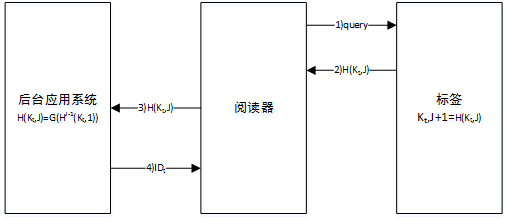
\includegraphics{chap3/hashChain.png}
	\caption{基本的RFID安全协议性能分析}\label{fig:Hash链协议图示}
\end{figure}

1)当阅读器的识别范围内有电子标签进入时,阅读器向其发送query消息请求认证。

2)电子标签利用Hash函数加密密钥K$_{t}$,J(即H(K$_{t}$,J))发送给阅读器,同时更新当前的密码值K$_{t}$,J+1=H(K$_{t}$,J)。

3)阅读器收到电子标签发送来的H(K$_{t}$,J)继而转发给后台应用系统。

4)后台应用系统查找数据库搜索存储的所有标签,计算是否有某个标签的ID$_{t}$使得H(K$_{t}$,J)=G(H$^{J-1}$(K$_{t}$,1)),若有,认证通过,并把ID$_{t}$发送给电子标签。否则认证失败。

选择Hash链协议的原因首先在于它每次都使用Hash函数更新发送给阅读器的信息,这点可以类比到Trivium算法每轮产生一个密钥上,还有就是在标签和后台应用系统之间共享了一个初始密钥K$_{t}$,1,这点可以类比到Trivium算法的密钥和初始向量,因此Hash链协议可以简单地把Hash函数替换成Trivium算法来加以实现。

改造后的协议如图\ref{fig:Trivium链协议图示}所示。

\begin{figure}[!htp]
	\centering
	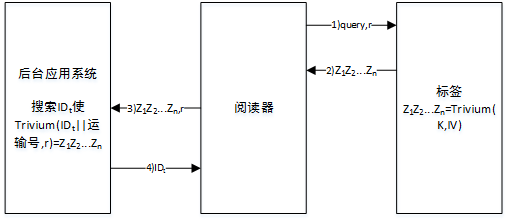
\includegraphics{chap3/triviumChain.png}
	\caption{基本的RFID安全协议性能分析}\label{fig:Trivium链协议图示}
\end{figure}

1)当阅读器的识别范围内有电子标签进入时,阅读器向其发送query消息请求认证。

2)电子标签根据密钥和初始向量运行一轮Trivium,更新自己的内部状态并输出这轮的密钥Z$_{J}$。

3)阅读器收到电子标签发送来的密钥Z$_{J}$继而转发给后台应用系统。

4)后台应用系统查找数据库搜索存储的所有标签,计算是否有某个标签的ID$_{t}$使得运行J轮后Trivium算法输出的密钥能等于密钥Z$_{J}$,若有,认证通过,并把ID$_{t}$发送给电子标签。否则认证失败。

\subsubsection{Trivium版RFID协议}

根据上节介绍的使用Trivium算法代替Hash链的RFID协议实现思路,尚存两个问题,第一个问题是具体到贵重物品追踪中,具体的硬件分配及所在位置,另一个问题是Trivium算法中密钥K和初始向量IV如何选择。

首先是硬件的问题,RFID协议涉及到三个硬件,分别是:后台应用系统、阅读器、标签,其中阅读器和标签的位置在之前已经提过,分别是在车内和物品上,那么问题就在于后台应用系统应该放在哪,一种选择是也放在车里,另一种自然是放在远程的数据中心。其实,只要看一下应用场景就可以知道是选择第一种。首要原因是使用RFID标签的目的是为了确定是否车内每一样物品都仍处于在车内的状态,这就要求需要阅读器周期性地扫描标签,并借由多个阅读器的定位确定标签的位置范围以确认标签是否在车内,因此这些阅读器本身需要一个统和的设施管理,于是后台应用系统就可以担任这个工作,每次认证通过后,阅读器再将与标签的距离信息发送给后台应用系统,然后后台应用系统根据所有阅读器对同一标签的距离计算出标签所在位置确认是否在车内。另一个原因是如果把后台应用系统放在远程,那还要考虑远程通信的方法,一种是随车辆的GPS信息一起发送,另一种是通过网络。但是随车辆的GPS信息发送的话,就要求GPS设备的厂商提供的开发接口能够实现发送用户自定义消息的功能,这点基本而言就已经不可能了,何况即使发出去,也没法接收。而通过网络的话,会有信号状态和延时问题。首先是延时,既然是远程通信那肯定要建立连接,而建立连接本身就会消耗很多时间,其次网络传输会有丢包问题,不断地超时重发,极可能到下一个检测周期,上一个检测周期的数据还没发出去,这时候就会产生误报发生物品丢失的情况。关键还在于信号问题,起码现在,在隧道这种地方信号都是很差的,而运输业走隧道的可能性还是很高的,不可能因为为了防止信号不好就让运输车绕远路,这反而是一种本末倒置,更何况现在也不是世界各地每个地方都有无线网覆盖,从起点到终点要选择一条全程被无线网覆盖的路线也不是一件轻松的事。所以综合考虑,还是直接将后台应用系统也放在车内比较合适。


